%%%%%%%%%%%%%%%%%%%%%%%
%%      Lecon 3      %%
%%%%%%%%%%%%%%%%%%%%%%%

\chapter{Récession : de la crise de la finance vers celle des Etats}
\section{Résumé jusqu'ici}
Si on doit faire le résumé des 2 premiers chapitres : 
\begin{itemize}
	\item \textbf{La finance a radicalement changé en 20 ans} : Crédits risqués et endettements des ménages, innovations financière et effet de levier, course à la rentabilité, fragentation du métier bancaire.
	      
	\item \textbf{Exhubérance irrationnelle :} On est en pleine euphérie irrationnelle c'est à dire qu'on est dans nos dreams on pense que tout ira bien et on fait des hypothèses très optimistes.
	      
	\item \textbf{Puis perte de confiance :} des épargnants, des actionnaires, des autres banques et du personnel. 
	      
	\item \textbf{Faillite de grandes banques :} on ne pensait pas que c'était possible. 
	      
	\item \textbf{On se tourne vers les Etats :} plus rien ne va donc les risques et profits privés deviennent publics au détriment de l'endettement des Etats.  
\end{itemize}

\section{Mesure en économie - frêt maritime}
On a par exemple le \textbf{Dry Baltic Index} (BDI) originaire de Virginia and Baltick Coffeehouse. \footnote{Londres - Financial District (1744)} Le fonctionnement est simple, les courtiers en fret maritime récoltent tous les jours et dans le monde entier les prix du frêt et on calcul un indice global qui sera publié.\\
Cette indicateur à ses inconvénients et montrons les dans le cadre du transport maritime. Le BDI fluctue très fort en cas de déséquilibre offre-demande. En effet, la demande peut varier du jour au lendemain mais l'offre ne sait pas suivre (les bateaux sont là). Ceci entraine de grands changements de prix avec la demande. Elle ne permet pas de prévoir l'économie mais permet de voir les tendance du commerce mondial (de biens matériels). 

\begin{wrapfigure}[10]{l}{9cm}
	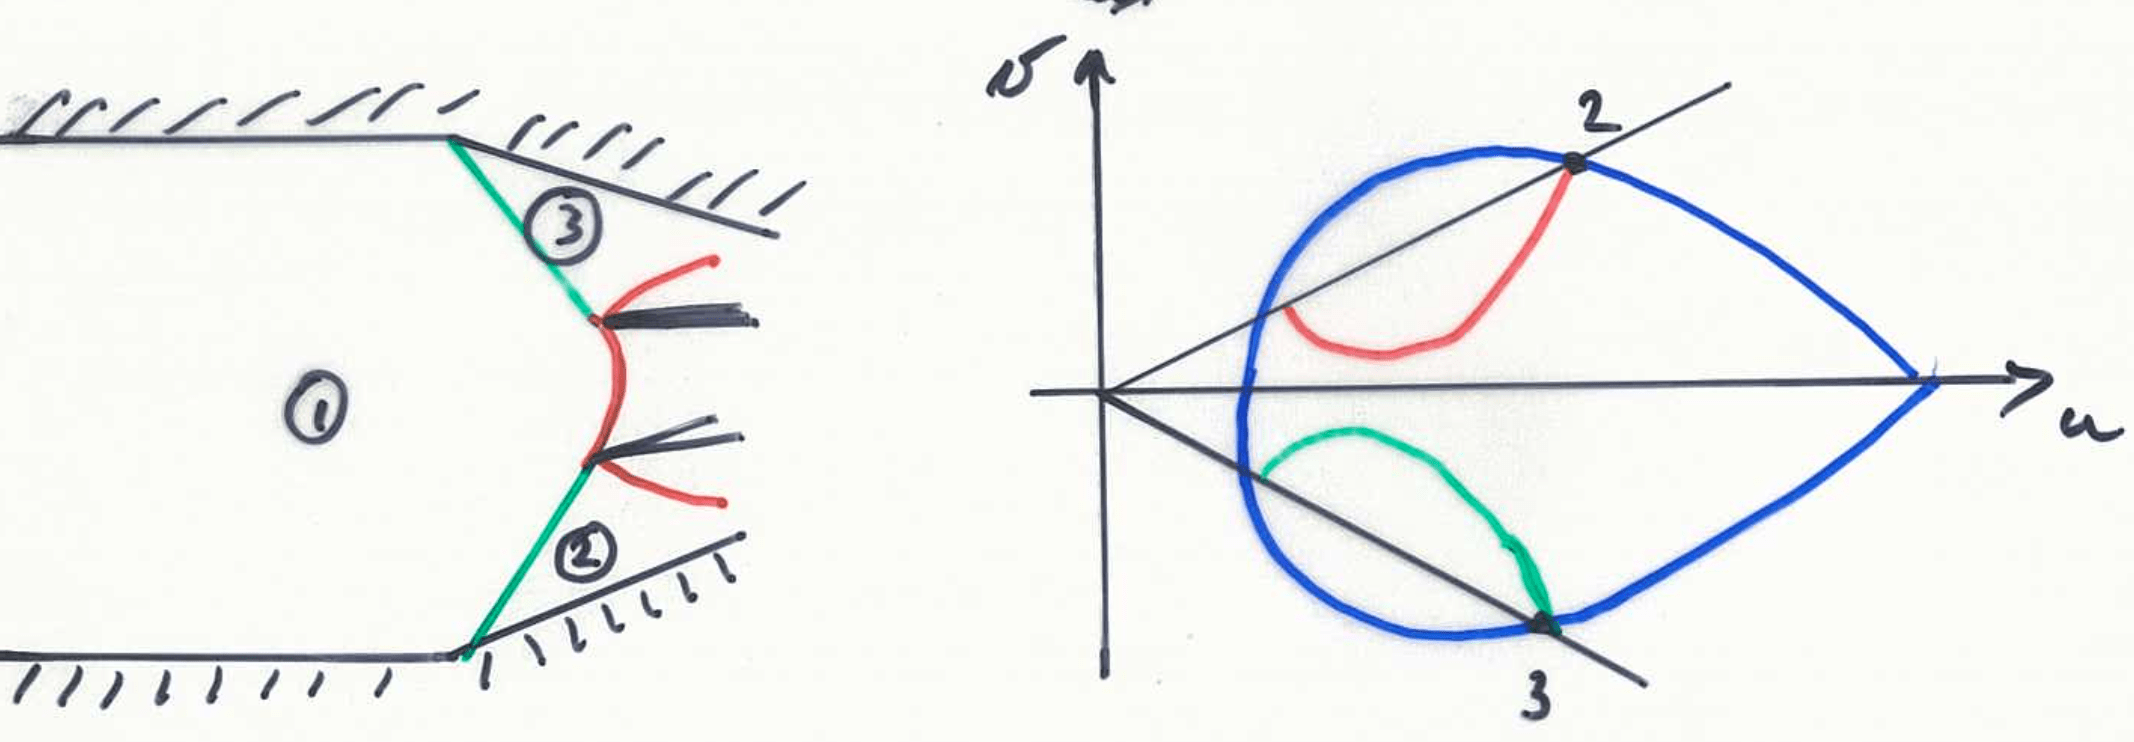
\includegraphics[scale=0.3]{14}
\end{wrapfigure}  
Regardons maintenant le BDI pour le frêt maritime (à gauche). Comme on peut le voir, les prix se sont effondrés en 2008. Comment est-ce qu'on adapte l'offre dans ce cas là ? Parce que si le marché monte trop, ça attire les investisseurs et donc ça favorise l'achat de nouveaux bateaux. C'est ce qui se passe dans notre graphe et c'est très mauvais pour la chute subite. \\
Solutions : A long terme, on peut reporter ou annuler les commandes aux chantiers navals ou même envoyer les vieux bateaux à la casse. A moyen terme, on doit mettre les navires à l'ancre (ne travaillent pas) mais beaucoup d'entreprises font faillite. A court terme, on diminue la vitesse des bateaux pour réduire la capacité et on économise ainsi du fuel. 

\section{La chaîne de la crise}
\begin{wrapfigure}[8]{l}{9cm}
	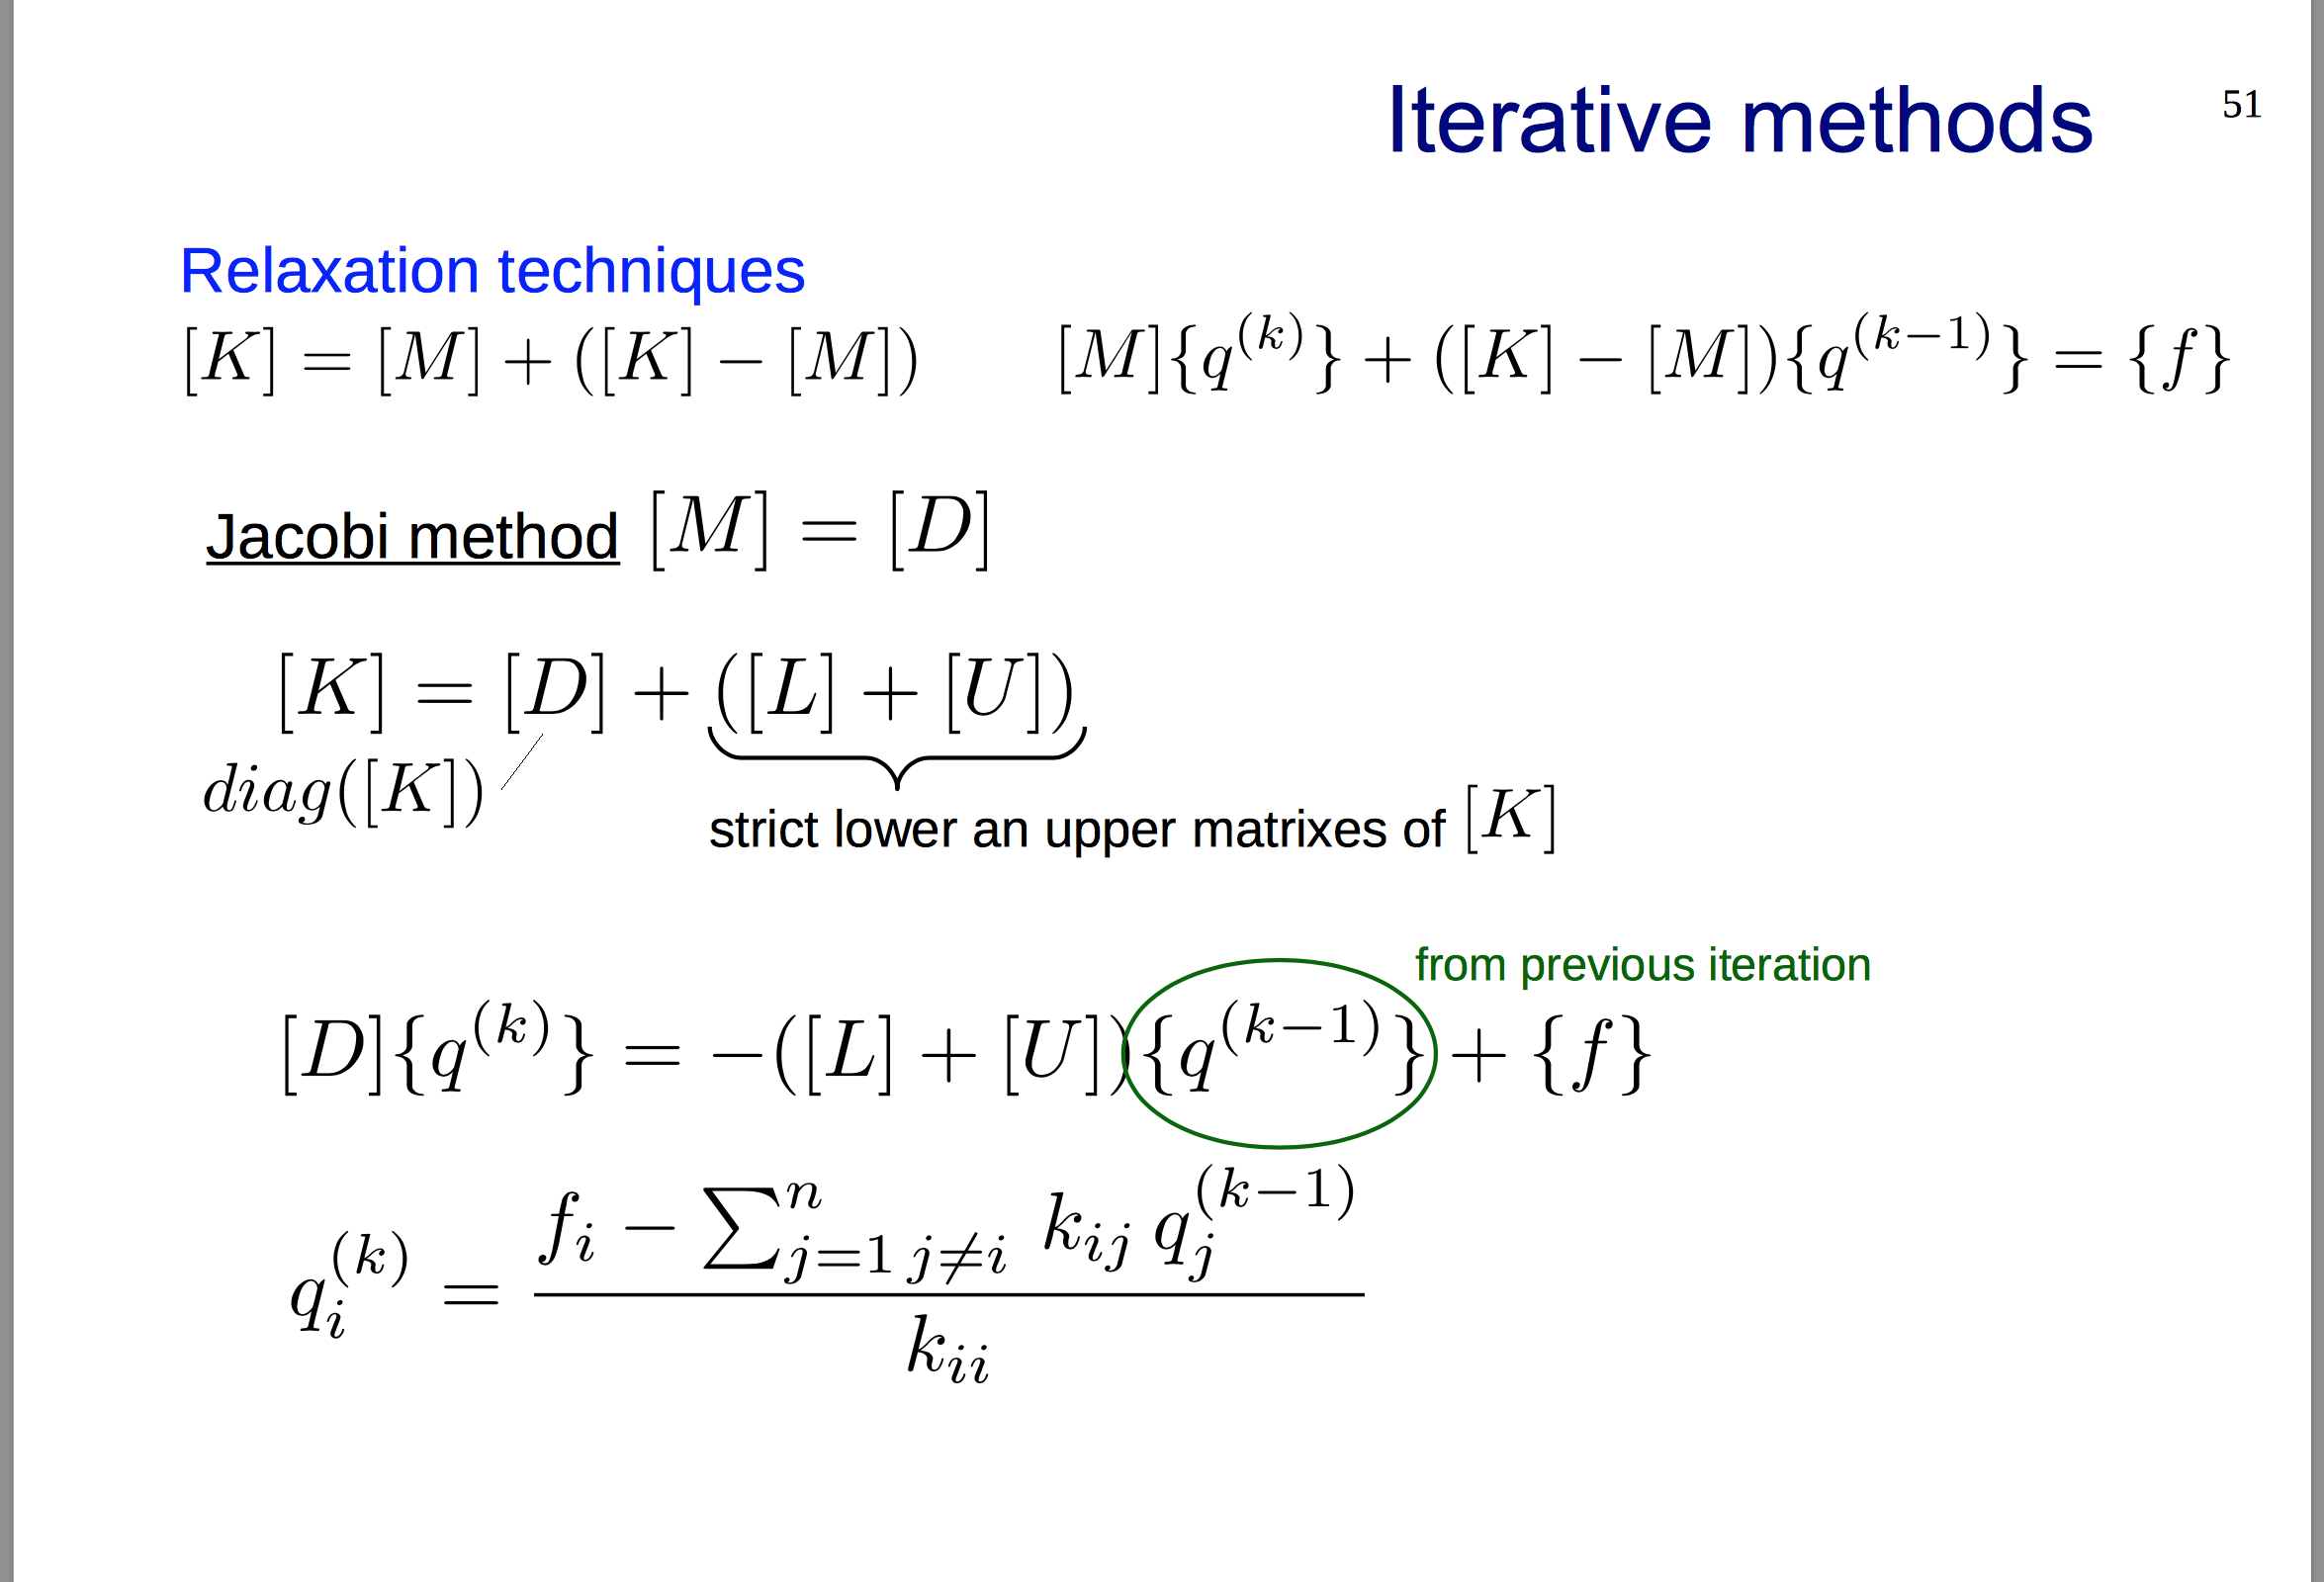
\includegraphics[scale=0.3]{15}
\end{wrapfigure}
Comme on l'a vu dans les chapitres précédents, tout à commencé par la finance. Un résumé en ligne du temps est présenté à la figure ci-dessous. Nous allons voir maintenant comment la crise de la finance s'est manifesté dans les autres secteurs, notamment dans l'industrie automobile.\\\\

\subsection{Crise dans l'industrie}

\begin{wrapfigure}[12]{l}{9cm}
	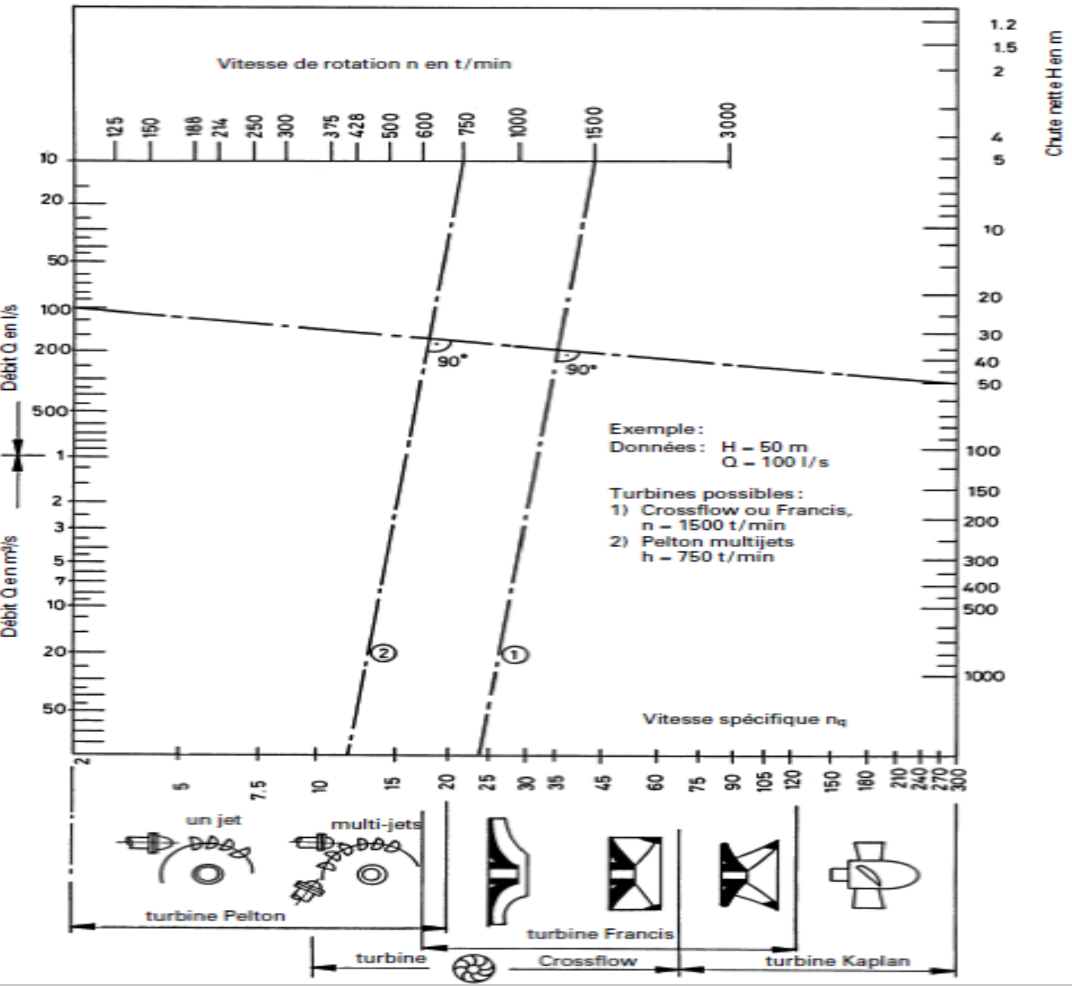
\includegraphics[scale=0.3]{16}
\end{wrapfigure}
\ \\ Comme on peut le voir sur la figue ci-contre, le secteur automobile se porte très mal. On voit que la vente d'automobile en 2008 et 2009 est bien plus faible qu'en 2007 et qu'elle s'accentue au fil des mois. De plus, tous les pays ne sont pas touché de la même manière. Par exemple, en janvier 2009, on observe une chute de -27\% réparti en : Espagne -41.6\% , UK -30.9\% , Belgique -16.1\% et la France -7.9\% .\\
Bien sûr ce n'est pas le seul secteur touché. Tous les types de bien et tous les fabricants sont touchés mais pas de la même façon : pneus Michelin -15.0\% , GSM -5.0\% mais Nokia -15.0\% , ... On a donc une véritable chute de la demande de biens durables. 

\begin{wrapfigure}[11]{l}{9cm}
	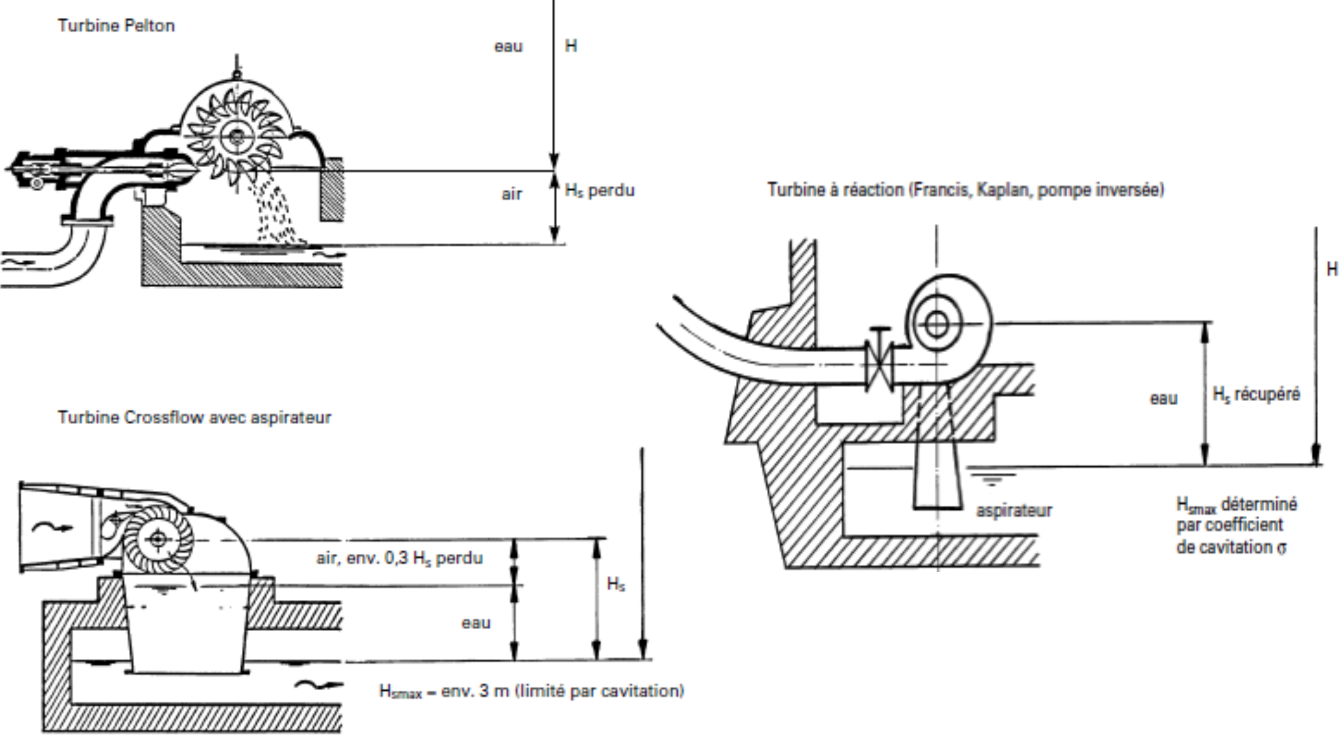
\includegraphics[scale=0.3]{17}
\end{wrapfigure}
Quelle est la réaction des entreprises ? Elles vont évidemment essayer de se protéger et vont réduire leur production de telle manière à arriver en fin 2008 à baisser la production beaucoup plus par rapport à la baisse des immatriculations. Ceci a pour conséquences des licenciements, des chômages techniques et une cessession d'embauche qui limite encore plus le pouvoir d'achat. De plus, les entreprises diminue fortement leur investissements dans la construction de nouveaux lieux de travail et donc la nous sommes dans un cercle vicieux puisque le même processus que dans le secteur automobile se manifestera (demande $\searrow$ production $\searrow$ frêt $\searrow$ emploi $\searrow$ ).

\begin{wrapfigure}[11]{l}{9cm}
	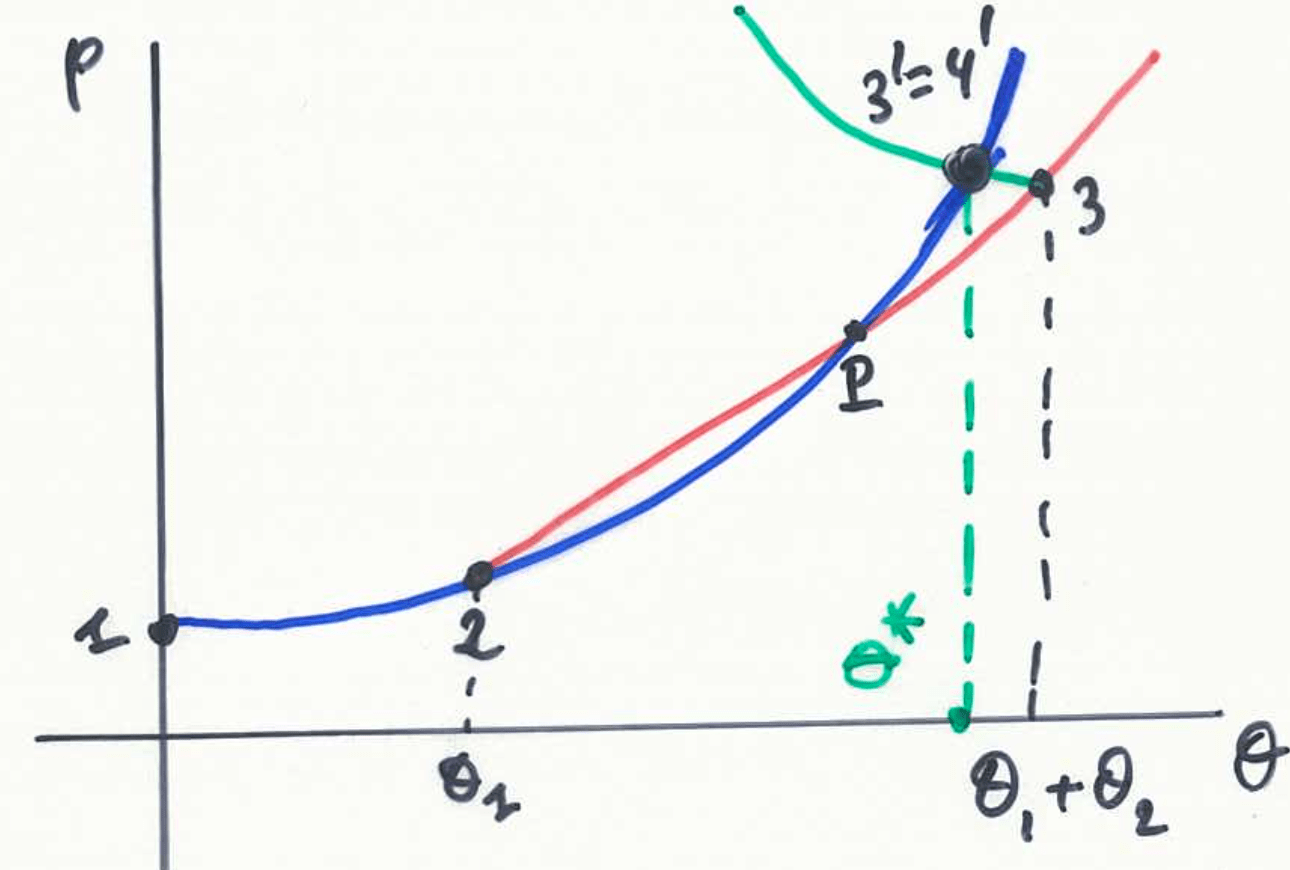
\includegraphics[scale=0.3]{18}
\end{wrapfigure}
La crise que nous observons commence à se manifester dans tous les pays. On peut voir que l'Allemagne, dont l'économie est fortement influencé par l'automobile et les machines, possède la plus grosse baisse de PIB. Cependant, cette crise commence à toucher le monde entier. En effet, les pays d'Asie qui exportent énormément vers l'Europe et les USA vont voir celles-ci chuter. Par exemple, Taiwan perd 42\% de ses exportations, l'Inde 22\%, etc. (graphique slide 4). La crise mène donc à une dépression économique mondiale ! 
\begin{center}
	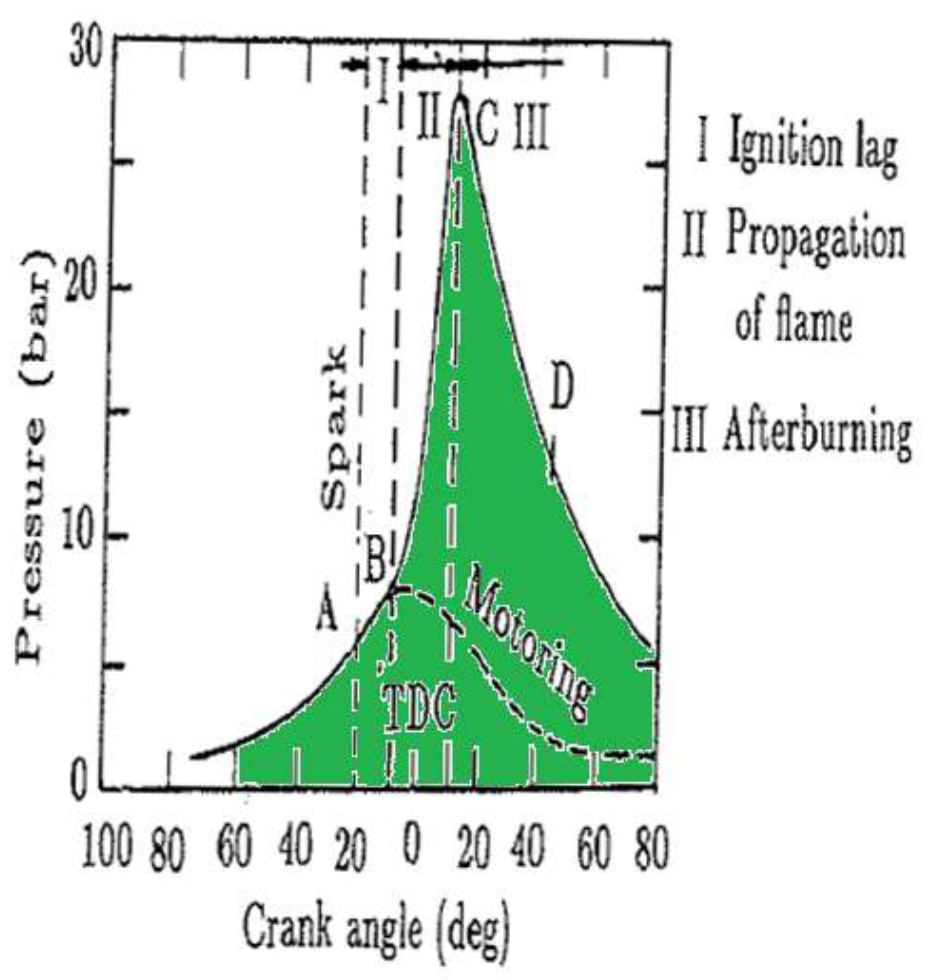
\includegraphics[scale=0.4]{19}
\end{center} 
\subsection{Crise des matières premières}
La matière première la plus importante est l'acier puisque c'est le composant de base pour les biens durables et d'investissement. Si on regarde le premier graphique, en 2006, on a une explosion de la demande notamment grâce à la croissance excellente de la Chine et l'Inde. Seulement, avec tout le processus de crise, la demande chute jusque 25\% par rapport à l'année précédente. C'est la plus grosse chute après la WW2. Ceci se généralise à toute forme de matière première. Le prix du baril de pétrole (fort indicateur pour l'économie mondiale) s'effondre en 2008 ! On voit de nouveau ce phénomène de forte croissance juste avant la chute (v. 2$^{ème}$ graphique).
\\\\
\begin{minipage}{0.55\textwidth}
	\begin{flushleft}
		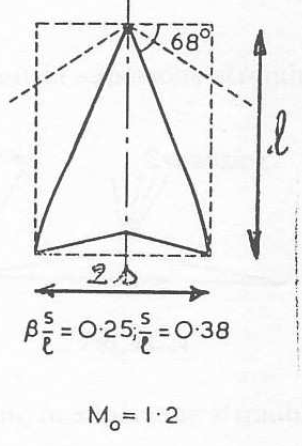
\includegraphics[scale=0.28]{20}
	\end{flushleft}
\end{minipage}
\begin{minipage}{0.5\textwidth}
	\begin{flushright}
		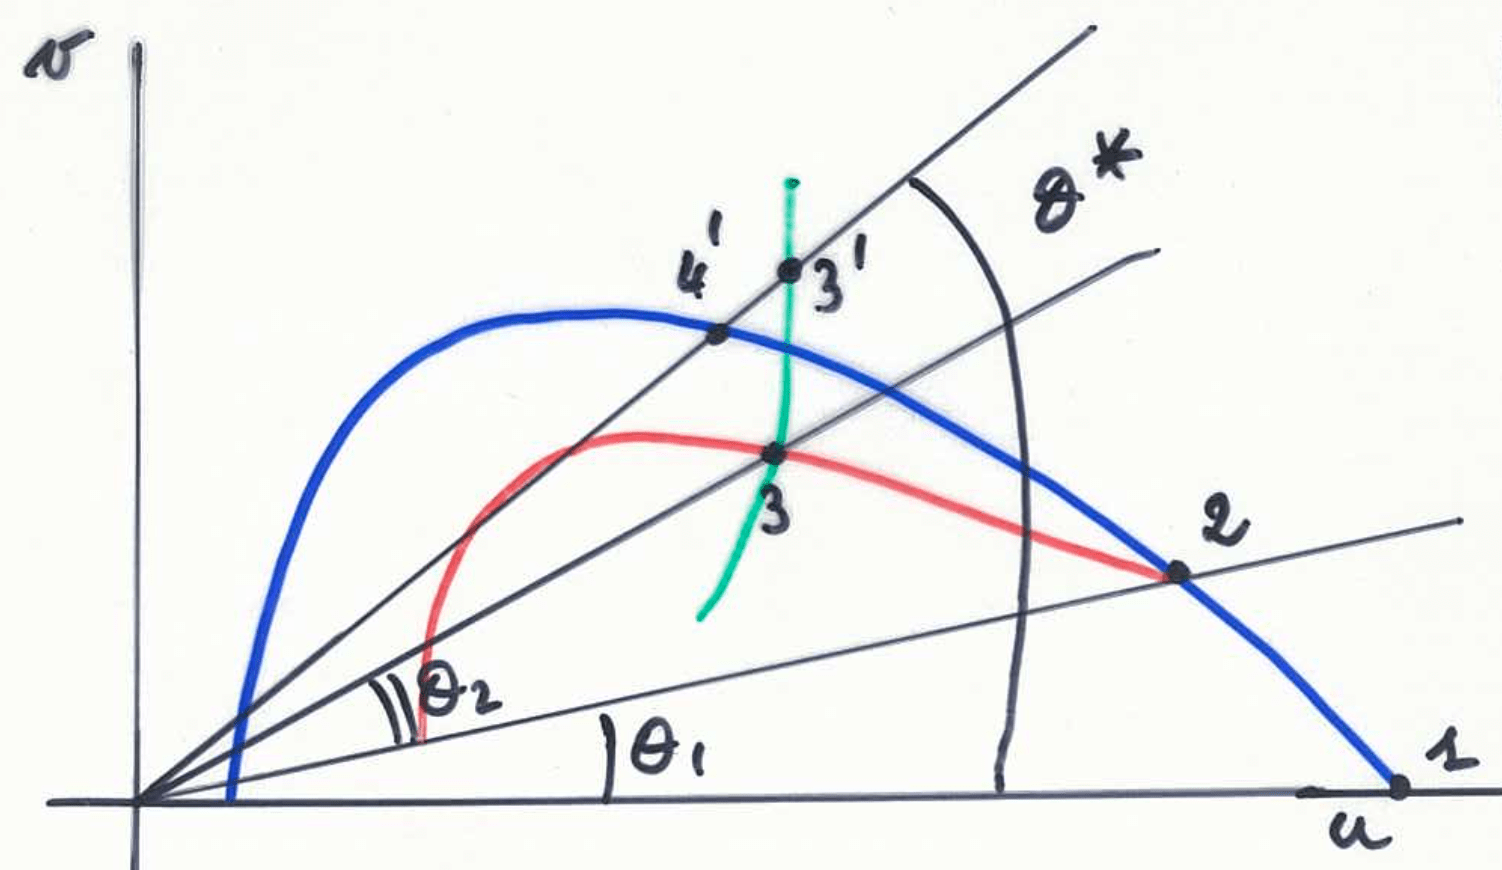
\includegraphics[scale=0.3]{21}
	\end{flushright}
\end{minipage}
\\\\
La mondialisation fait en sorte que la crise prend une plus forte empleur et devient de plus en plus conséquent puisque le cercle viscieux s'aggrave et n'est pas prêt de s'arrêter puisque les consommateurs perdent toujours leur confiance. 

\begin{center}
	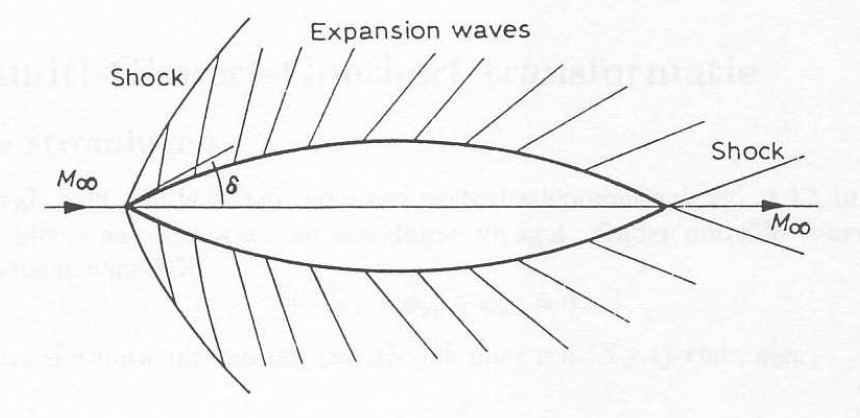
\includegraphics[scale=0.4]{22}
\end{center}

\section{Actions de sauvetage}
\subsection{Dégradation des prévisions}
\begin{wrapfigure}[13]{l}{9cm}
	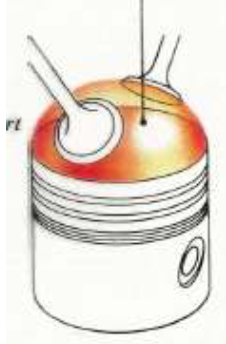
\includegraphics[scale=0.35]{23}
\end{wrapfigure}
Le rêve de tout économiste est de pouvoir prédir le cours de la finance. C'est très compliqué parceq que des événements se produisent tous les jours et influe cette dernière. Cependant, certains expert essaye d'anticiper les évolutions futures d'après les modèles qu'ils établissent. Ca permet à tout le monde de se faire une idée avant d'investir. Voici ci-dessous une prévision pour le PIB de certains états. On peut voir que la \textbf{faillite de Lehman Brothers} a provoqué un tournant dans les prévisions et les économistes ne sont plus très optimistes pour la suite. En effet, la crise fait perdre confiance à tout le monde, la demande et la production de biens durables chute, les investissements aussi, le pouvoir d'achat baisse à cause des pertes d'emploi et reprend la boucle du début. Comment éviter une crise comme en 1929-30 ?

\subsection{La crise économique évitée}
A partir de février 2009 jusqu'en fin 2010, les Etats ont mené des actions rigoureuses et coordonnées. De plus, plus le temps avance, plus on a de nouveaux besoin. Donc on peut accéder à de nouveaux marchés en innovant. L'immobilier reprend petit à petit et on essaye de désendetter les ménages et leur permettre une épargne. Tout ça permet de briser la chaine de récession et les premiers signes de reprise apparaissent. C'est l'Asie qui sort en premier de ce cercle viscieux et a déjà presque oublié la récession. Cependant, on a éviter la crise au détriment des Etats qui se sont endettés lourdement. Nous allons tout droit vers la crise des Etats !

\subsection{Etat des lieux et évolution après dépression}
\begin{wrapfigure}[8]{l}{8cm}
	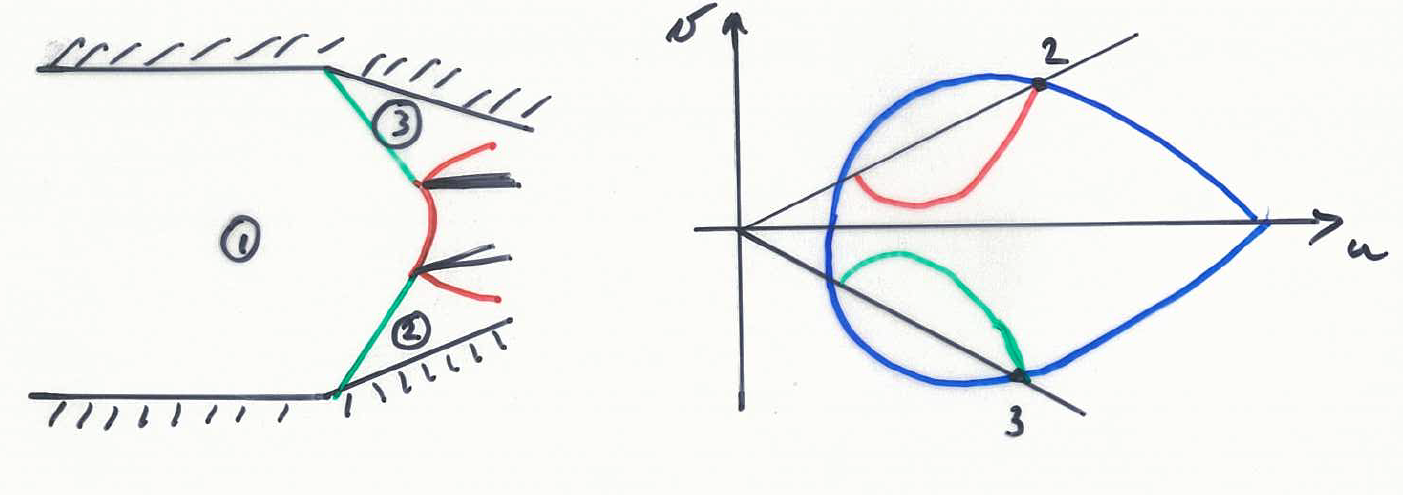
\includegraphics[scale=0.28]{24}
\end{wrapfigure}
\ \\ Comme on l'a cité juste au point précédent, les Etats s'endettent lourdement. Si on regarde l'évolution jusqu'en 2011 de la dette greque, on peut confirmer la crise de cet Etat, alors qu'on pensait que les Etat ne pouvvait pas faire faillite. La Grèce a divisé les opignons en deux (Grexit or No Grexit). 

\begin{wrapfigure}[6]{l}{8cm}
	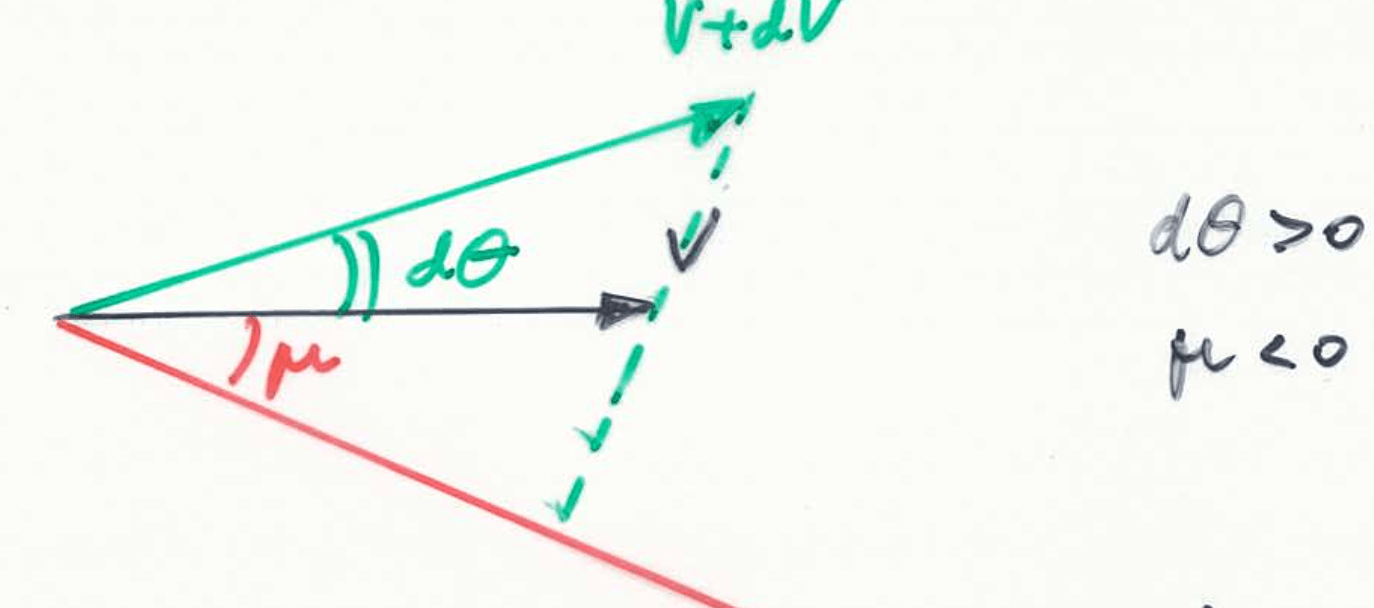
\includegraphics[scale=0.26]{25}
\end{wrapfigure}
\ \\ Aussi, on a peut-être évité une crise, mais l'économie mondiale ne s'en est pas remis après ces événement. La Dry Baltic Index, nous montre une stagnation du prix du frêt et donc un équilibrage des échanges inter-Etats. \\\\

\begin{wrapfigure}[9]{l}{9cm}
	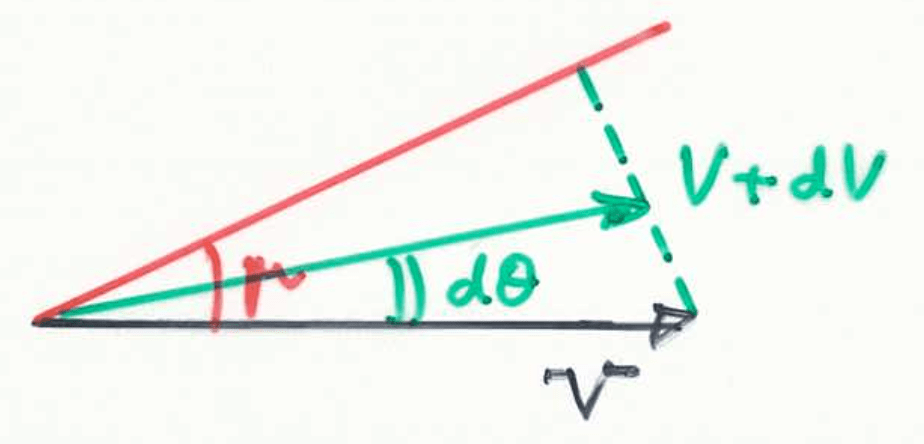
\includegraphics[scale=0.32]{26}
\end{wrapfigure}
\noindent Par contre, on observe sur ce graphique que l'Asie s'est très bien tiré de l'affaire et a provoqué un changement du centre de gravité de l'économie mondiale. Les grandes puissances auparavant qui étaient les Etats-Unis et certains pays d'Europe, laisse la place à la \textbf{BRIC} (Brésil, Russie, Inde, Chine) auquel on peut inclure l'Afrique du Sud.  